\documentclass{beamer}
\mode<presentation>
\usepackage[utf8]{inputenc}

\usetheme{Luebeck}
\usecolortheme{dolphin}
\setbeamertemplate{footline}[frame number]
\setbeamertemplate{caption}[numbered]
\setbeamertemplate{navigation symbols}{}
\setbeameroption{hide notes}
\setbeamertemplate{note page}[plain]
\usepackage[english]{babel}%Set language as english%
\usepackage[babel]{csquotes}%Nicer quotations%
\usepackage{indentfirst}
\usepackage[protrusion=true,expansion=true]{microtype}
%Math Formatting%
\usepackage{amsmath}%AMS Math%
\usepackage{amsthm}%Theorem Formatting%
\usepackage{amssymb}%AMS Symbols%
\usepackage{array}%Allows for more complex matrices
\usepackage{siunitx}%Formats SI units%
\DeclareSIUnit{\molar}{M}%Adds molarity as unit%
\usepackage{booktabs}%Typsets tables%
\newcommand{\specialcell}[2][c]{\begin{tabular}[#1]{@{}l@{}}#2\end{tabular}}
\newcommand{\specialcellbold}[2][c]{%
	\bfseries
	\begin{tabular}[#1]{@{}l@{}}#2\end{tabular}%
}
\usepackage{chemformula}%Typsets Chemical Formulas$
%Image Formatting%
\usepackage{graphicx}%Enchanced graphics support%
\usepackage{media9}
\graphicspath{{./figures/}}
\usepackage{float}%Float options$

\usepackage[
backend=biber,
style=chem-acs
]{biblatex}
\addbibresource{references.bib}

\title{Application of Mathematical Methods in the Study of Chemical Dynamical Systems to an Inventory Multiplier-Accelerator Business Cycle Model}
\author{Benjamin Bui}
\date{May 3, 2019}
\begin{document}
\begin{frame}
	\titlepage
\end{frame}

\section{Introduction}
\begin{frame}{Motivation}
	\begin{columns}
	\begin{column}{0.5\textwidth}
	\begin{itemize}
		\item The study of stochastic processes was deeply influential in explaining macroscale themodynamic properties

		\item Although first applied by French mathematician Louis Bachelier\autocite{Bachelier1900}, Einstein popularized the application of stochastic processes which helped its spread into the fields of finance and economics
	\end{itemize}
	\end{column}
	\begin{column}{0.5\textwidth}
		\begin{figure}
			\centering
			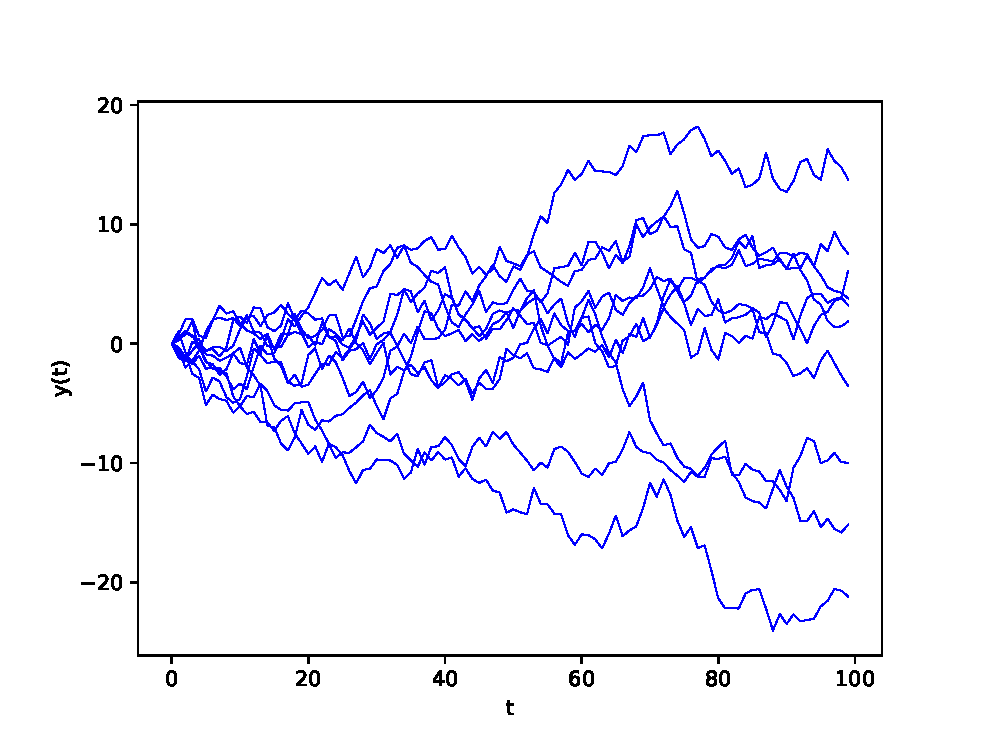
\includegraphics[width=0.9\textwidth]{brownian_motion.eps}
			\caption{Discrete brownian motion of a 10 independent particles over 100 iterations with a mean of 0 and a standard deviation of 1.}
		\end{figure}
	\end{column}
	\end{columns}
\end{frame}
\note{Brownian motion, a stochastic evolutionary process, laid the framework for the study of statistical mechanics which bridged the gap between the behavior and interactions of individual particles and the thermodynamic properties of the constituent material.}
\begin{frame}{Motivation}
	\begin{columns}
	\begin{column}{0.5\textwidth}
		\begin{itemize}
			\item Fractals and chaotic processes are a more recent addition to the chemist's toolkit\autocite{Beutel2007,Morris2010}
			\item Could chaos play a role in economics as well?
		\end{itemize}
	\end{column}
	\begin{column}{0.5\textwidth}
		\begin{figure}
			\centering
			\includegraphics[width=0.9\textwidth]{bz_reaction.jpg}
			\caption{Still image of the BZ-reaction}
		\end{figure}
	\end{column}
	\end{columns}
\end{frame}
\note{Fractals and chaos theory are common in physical dynamical systems but are increasing in popularity in chemistry for their ability to model and explain cyclic processes like the BZ-reaction. They have seen less attention than stochastic dynamical systems, only reaching prominence in the 1960s. It has played an important role in providing accurate models describing flame dynamics, electrochemical deposits, surface chemistry, and self-replicating molecules.}
% \begin{frame}{Overview}
% 	\begin{itemize}
% 		\item Wegener et al.: Inventory cycle model with a Lundberg lag
% 		\item T\"onu Puu: Multiplier-acclerator growth model with a Robertson lag
% 		\item Benjamin Bui: Inventory Cycles with endogenous investment
% 	\end{itemize}
% \end{frame}
\section*{Inventory Cycles}
\begin{frame}{Background}
	\begin{itemize}
		\item Lloyd Metzler developed an inventory cycle model in 1941 in order to explore the effect of a Lundberg lag\autocite{Metzler1941}
		\item Wegener, Westerhoff, and Zaklan expanded on this model in 2009\autocite{Wegener2009}
	\end{itemize}
\end{frame}
\note{This model provided an endogenous, deterministic explanation for the dynamic nature of business cycles. It utilizes the Lundberg lag which means theres a discrepancy between goods demanded and goods produced. This disagrees with Classical market clearing theories which assume that supply will always equal demand and that agents will behave with perfect rationality.}
\begin{frame}{Consumption and Investment}
	\begin{columns}
	\begin{column}{0.5\textwidth}
		\begin{itemize}
			\item Investment is held as endogenous 
			\item Consumption is a proportion of income
		\end{itemize}
	\end{column}
	\begin{column}{0.5\textwidth}
		\begin{align*}
			I_t &= \bar I\\
			C_t &= bY_t
		\end{align*}
	\end{column}
	\end{columns}
\end{frame}

\begin{frame}{Inventory}
	\begin{columns}
	\begin{column}{0.5\textwidth}
		\begin{itemize}
			\item Desired inventory, $\hat Q$ is a proportion of expected consumption
			\item Stock output, $S$ is made to match desired inventory
			\item Actual inventory, $Q$ depends on the accuracy of the expectation
			\item 
		\end{itemize}
	\end{column}
	\begin{column}{0.5\textwidth}
		\begin{align*}
			\hat Q_t &= kU_t\\
			S_t &= \hat Q_t - Q_{t-1}\\
			Q_t &= \hat Q_t - (C_t-U_t)
		\end{align*}
	\end{column}
	\end{columns}
\end{frame}

\begin{frame}{Predicting Consumption}
	\begin{columns}
	\begin{column}{0.5\textwidth}
		\begin{itemize}
			\item $U^E$: "Extrapolaters" believe that consumption will diverge from the steady-state
			\item $U^R$: "Regressers" believe that consumption will return to the steady-state
			\item Firms will choose from the types depending on the consumption level
		\end{itemize}
	\end{column}
	\begin{column}{0.5\textwidth}
		\begin{align*}
			U_t^E &= C_{t-1} + c(C_{t-1}-\bar C)\\
			U_t^R &= C_{t-1} + f(\bar C-C_{t-1})\\
			U_t &= w_tU_t^E+(1-w_t)U_t^R\\
			w_t &= \frac{1}{1+d(\bar C-C_{t-1})^2}
		\end{align*}
	\end{column}
	\end{columns}
\end{frame}

\begin{frame}{Aggregate Output}
	\begin{columns}
	\begin{column}{0.5\textwidth}
		\begin{itemize}
			\item Output, $Y$, is the sum of these production factors
			\item Can solve for a single fixed point
		\end{itemize}
	\end{column}
	\begin{column}{0.5\textwidth}
		\begin{align*}
			Y_t = I_t + U_t + S_t\\ 
			\bar Y = \frac{1}{1-b}\bar I
		\end{align*}
	\end{column}
	\end{columns}
\end{frame}

\begin{frame}{A Possible Trajectory}
	\begin{figure}
		\centering
		\includegraphics[height=0.7\textheight]{timeseries_income.eps}
		\caption{Timeseries with conditions: $Y_0=40.6,\ U_0=30.3,\ \bar I=10,\ b=0.75,\ c=0.3,\ d=1.0,\ f=0.1,\ k=0.1$}
	\end{figure}
\end{frame}

\section*{Multiplier-Accelerator}
\begin{frame}{Framework}
	\begin{columns}
	\begin{column}{0.5\textwidth}
		\begin{itemize}
			\item Consumption, $C$, has a Robertson lag
			\item Investment, $I$, is cubic relative to income change
			\item There is no Lundberg lag
		\end{itemize}
	\end{column}
	\begin{column}{0.5\textwidth}
		\begin{align*}
			C_t &= (1-s)Y_{t-1} + sY_{t-2}\\
			I_t &= v(Y_{t-1}-Y_{t-2})-v(Y_{t-1}-Y_{t-2})^3
		\end{align*}
	\end{column}
	\end{columns}
\end{frame}
\begin{frame}{The Growth Model}
	\begin{columns}
	\begin{column}{0.5\textwidth}
		Change in income is normalized\autocite{Puu2003} to be within the range (-1, 1)
	\end{column}
	\begin{column}{0.5\textwidth}
		\begin{align*}
			\mu &\equiv v-s\\
			\dot Y_t &= \mu\dot Y_{t-1}-(\mu+1)\dot Y_{t-1}^3
		\end{align*}
	\end{column}
	\end{columns}
\end{frame}

\begin{frame}{Qualitatively Different Trajectories Possible}
	\begin{columns}
	\begin{column}{0.5\textwidth}
		\begin{figure}
			\centering
			\includegraphics[width=1.2\textwidth]{2-cyclic.eps}
			\caption{Cobweb plot with conditions $\mu=2.15$ and $\dot Y_0=0.1$}
		\end{figure}
	\end{column}
	\begin{column}{0.5\textwidth}
		\begin{figure}
			\centering
			\includegraphics[width=1.2\textwidth]{chaos_uncontained.eps}
			\caption{Cobweb plot with conditions $\mu=2.6$ and $\dot Y_0=0.1$}
		\end{figure}
	\end{column}
	\end{columns}
\end{frame}

% \begin{frame}{Growth Dynamics}
% 	\begin{columns}
% 	\begin{column}{0.5\textwidth}
% 		\begin{figure}
% 			\centering
% 			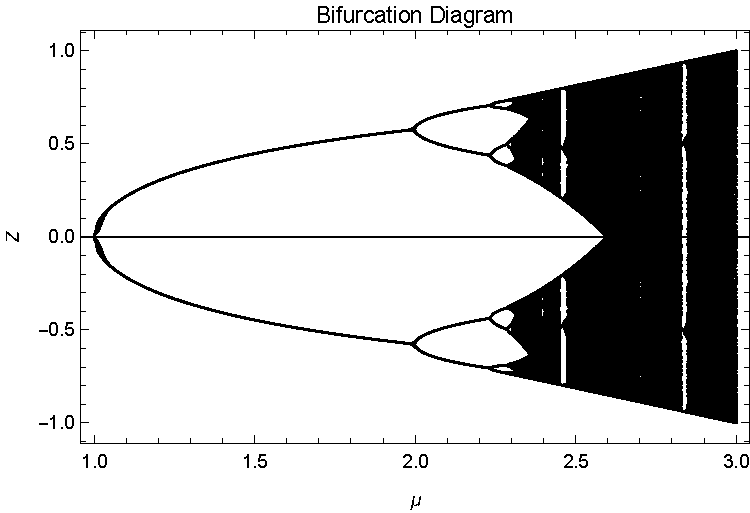
\includegraphics[width=1.2\textwidth]{bifurcation.eps}
% 		\end{figure}
% 	\end{column}
% 	\begin{column}{0.5\textwidth}
% 		\begin{figure}
% 			\centering
% 			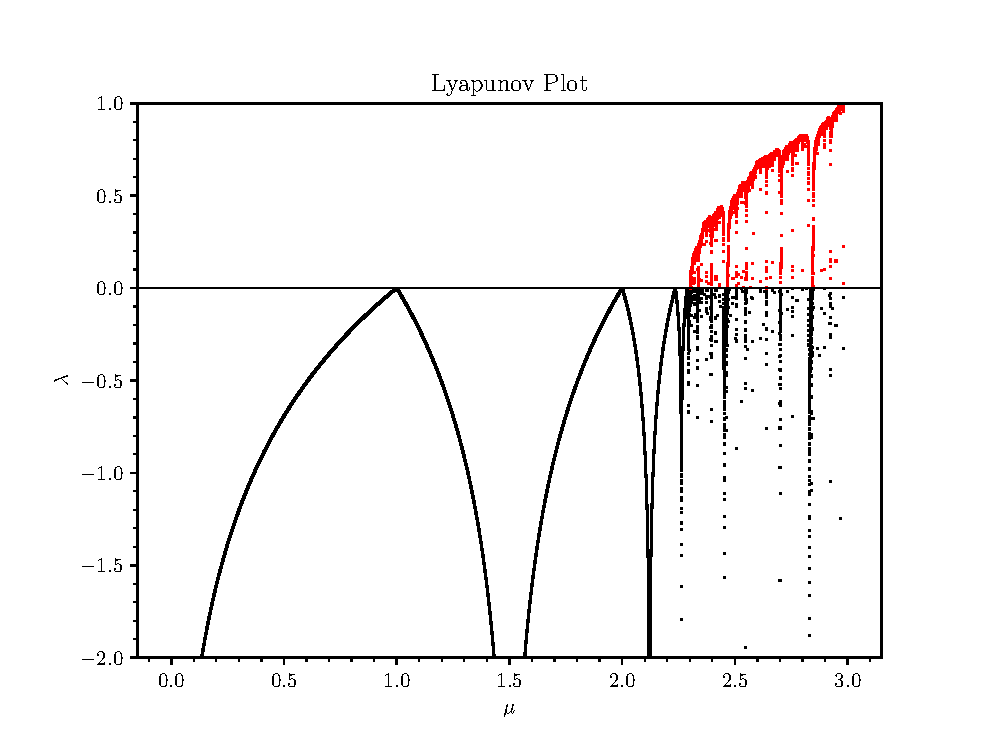
\includegraphics[width=1.2\textwidth]{lyapunov.eps}
% 		\end{figure}
% 	\end{column}
% 	\end{columns}
% \end{frame}

\section*{Inventory Cycle with Growth}
\begin{frame}{Goal}
	\begin{itemize}
		\item To incorporate a Robertson and Lundberg lag in the same model
		\item To provide a reasonable basis for the boundedly rational behavior of firms
	\end{itemize}
\end{frame}

\begin{frame}{Consumption and Investment}
	\begin{columns}
	\begin{column}{0.5\textwidth}
		\begin{itemize}
			\item Consumption, $C$, is identical to the multiplier-accelerator model
			\item The investment function, $I$, is qualitatively similar but asymptotically approaches 0
		\end{itemize}
	\end{column}
	\begin{column}{0.5\textwidth}
		\begin{align*}
			C_t &= (1-s)Y_{t-1}+sY_{t-2}\\
			I_t &= \frac{\frac{Y_{t-1}-Y_{t-2}}{v}}{\frac{Y_{t-1}-Y_{t-2}}{v}+q}
		\end{align*}
	\end{column}
	\end{columns}
\end{frame}

\begin{frame}{Investment Curve}
	\begin{figure}
		\centering
		\includegraphics[height=0.8\textheight]{investment.eps}
		\caption{Investment curve such that $v=500$ and $q=0.001$}
	\end{figure}
\end{frame}

\begin{frame}{Maximal/Minimal Investment}
	\begin{columns}
	\begin{column}{0.5\textwidth}
		\begin{align*}
			&Y_{t-1}-Y_{t-2} = \pm\frac{q^{1/4}v}{3^{1/4}}\\
			&I_t = \pm\frac{3^{3/4}}{3q^{3/4}}
		\end{align*}
	\end{column}
	\begin{column}{0.5\textwidth}
		\begin{figure}
			\centering
			\includegraphics[width=1.2\textwidth]{maxinvestment.eps}
			\caption{Plot of maximal investment relative to $q$.}
		\end{figure}
	\end{column}
	\end{columns}
\end{frame}

\begin{frame}{Investment FWHM}
	\begin{figure}
		\centering
		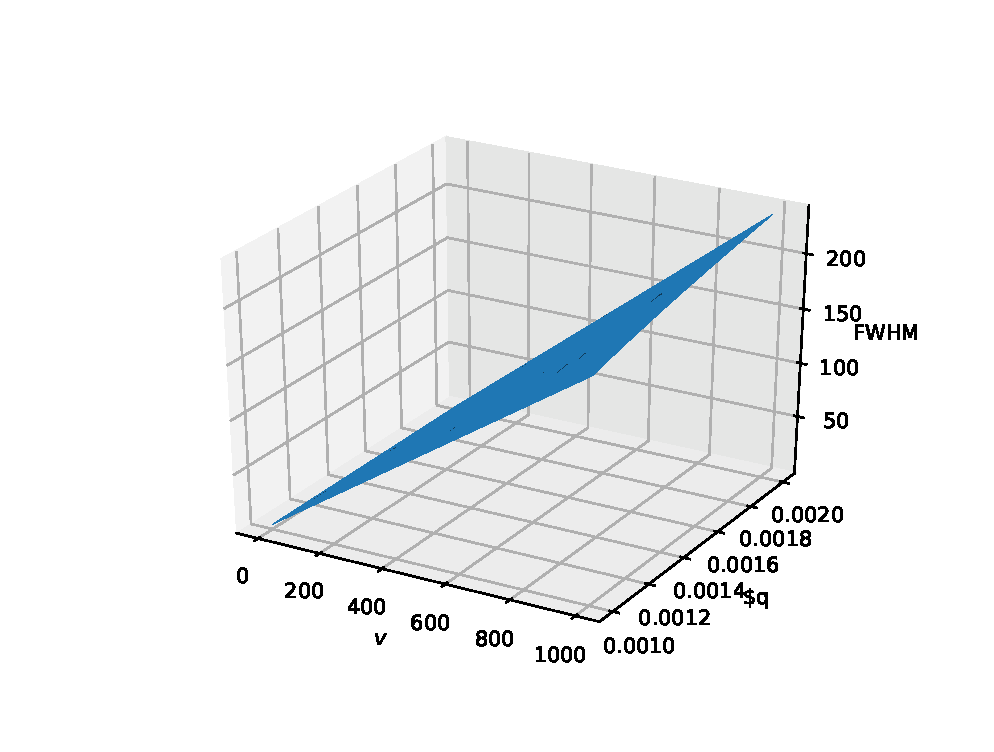
\includegraphics[height=0.8\textheight]{widthinvestment.eps}
		\caption{Triangulated plot investment FWHM relative to $v$ and $q$.}
	\end{figure}
\end{frame}

\begin{frame}{Inventory}
	\begin{columns}
	\begin{column}{0.5\textwidth}
		\begin{itemize}
			\item Predicted consumption, $U$, is an average of lagged consumption
			\item Evolution of stock output, $S$, and actual inventory, $Q$, behaves identically to the Wegener model
		\end{itemize}
	\end{column}
	\begin{column}{0.5\textwidth}
		\begin{align*}
			U_t &= \frac{C_{t-1}+C_{t-2}+C_{t-2}}{3}\\
			S_t &= kU_t-Q_{t-1}\\
			Q_t &= Q_{t-1} + S_t + (U_t-C_t)
		\end{align*}
	\end{column}
	\end{columns}
\end{frame}

\begin{frame}{Output Growth}
	\begin{columns}
	\begin{column}{0.5\textwidth}
		Endogenous investment allows for long-run growth or decay 
	\end{column}
	\begin{column}{0.5\textwidth}
		\begin{align*}
			Y_t &= I_t + S_t + U_t\\
			\dot Y_t &= Y_{t}-Y_{t-1}
		\end{align*}
	\end{column}
	\end{columns}
\end{frame}

\begin{frame}{Output Growth}
	\begin{equation*}
	\begin{split}
        \dot Y_{t}& = \frac{\frac{\dot Y_{t-1}}{v}}{\left(\frac{\dot Y_{t-1}}{v}\right)^4+q}-\frac{\frac{\dot Y_{t-2}}{v}}{\left(\frac{\dot Y_{t-2}}{v}\right)^4+q} + \\
		& \frac{k+1}{3}\left[(1-s)(\dot Y_{t-2}-Y_{t-5})+s(\dot Y_{t-3}-Y_{t-6})\right]\\
		& +(1-s)\dot Y_{t-2}+s\dot Y_{t-3}
	\end{split}
	\end{equation*}
\end{frame}

\begin{frame}{Possible Trajectories}
	\begin{columns}
	\begin{column}{0.5\textwidth}
		\begin{figure}
			\centering
			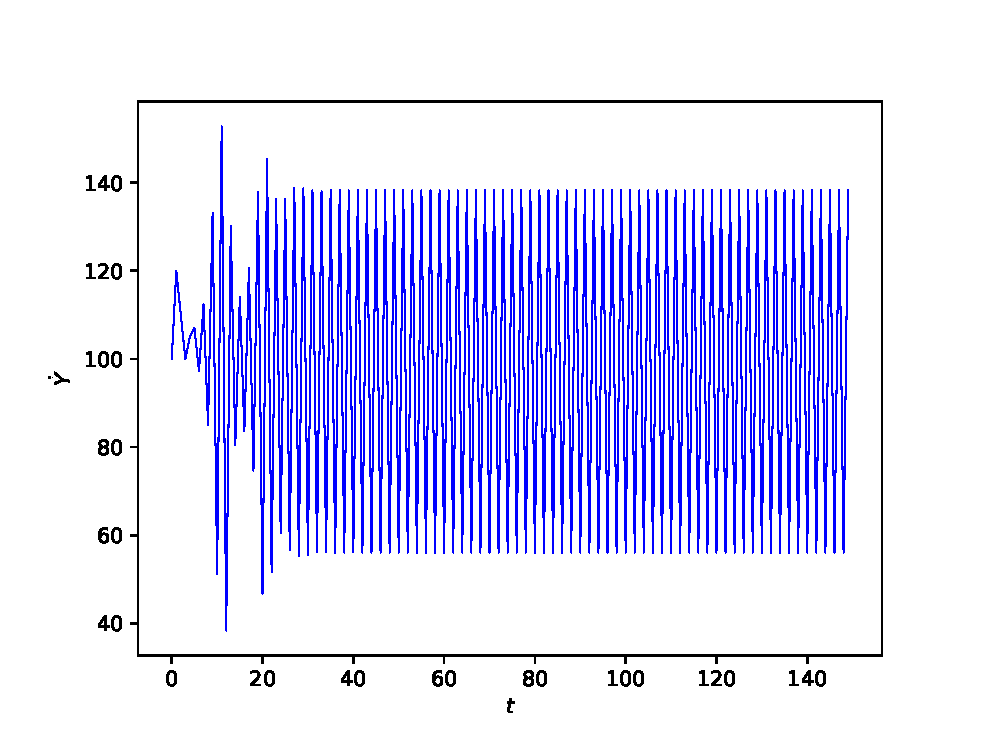
\includegraphics[width=1.0\textwidth]{timeseries1.eps}
			\caption{Timeseries plot with parameters: $s=0.6,\ k=0.3,\ v=500,\ q=0.001$. Initial values of $\dot Y$ are: 100, 120, 110, 100, 105, 107}
			\label{metzlerian_growth-timeseries1}
		\end{figure}
	\end{column}
	\begin{column}{0.5\textwidth}
		\begin{figure}
			\centering
			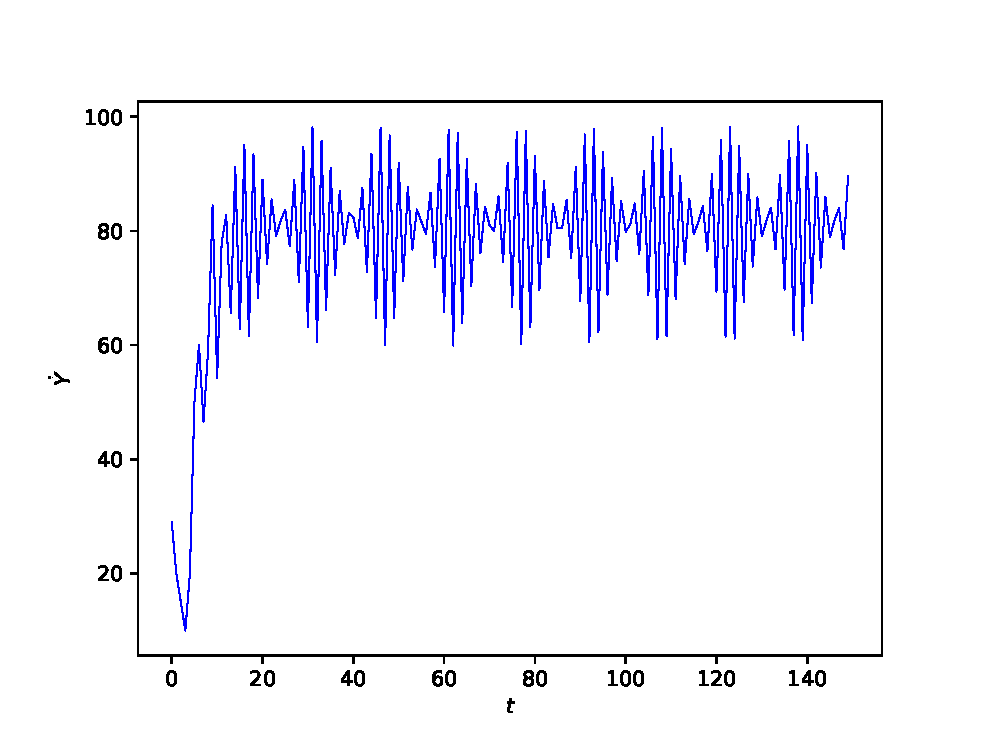
\includegraphics[width=1.0\textwidth]{timeseries3.eps}
			\caption{Timeseries plot of income growth rate over 150 iterations. Parameters identical to Fig. \ref{metzlerian_growth-timeseries1}. Initial values of $\dot Y$ are: 29, 20 , 15 , 10, 20, 50}
		\end{figure}
	\end{column}
	\end{columns}
\end{frame}

\begin{frame}{Determining Chaos}
	\begin{align*}
		\dot Y_t = f(\dot Y_{t-1}, \dot A_{t-1}, \dot B_{t-1}, \dot C_{t-1}, \dot D_{t-1}, \dot G_{t-1})\\
		\dot A_t = g(\dot Y_{t-1}, \dot A_{t-1}, \dot B_{t-1}, \dot C_{t-1}, \dot D_{t-1}, \dot G_{t-1})\\
		\dot B_t = h(\dot Y_{t-1}, \dot A_{t-1}, \dot B_{t-1}, \dot C_{t-1}, \dot D_{t-1}, \dot G_{t-1})\\
		\dot C_t = j(\dot Y_{t-1}, \dot A_{t-1}, \dot B_{t-1}, \dot C_{t-1}, \dot D_{t-1}, \dot G_{t-1})\\
		\dot D_t = l(\dot Y_{t-1}, \dot A_{t-1}, \dot B_{t-1}, \dot C_{t-1}, \dot D_{t-1}, \dot G_{t-1})\\
		\dot G_t = m(\dot Y_{t-1}, \dot A_{t-1}, \dot B_{t-1}, \dot C_{t-1}, \dot D_{t-1}, \dot G_{t-1})
	\end{align*}
\end{frame}
\begin{frame}{Determining Chaos}
	\begin{equation*}
		J=
		\begin{bmatrix}\small
			\frac{\partial f}{\partial Y_{t-1}} & \frac{\partial f}{\partial A_{t-1}} & s+\frac{k+1}{3}s & 0 & \frac{(k+1)(s-1)}{3} & -\frac{(k+1)s}{3}\\
			1 & 0 & 0 & 0 & 0 & 0\\
			0 & 1 & 0 & 0 & 0 & 0\\
			0 & 0 & 1 & 0 & 0 & 0\\
			0 & 0 & 0 & 1 & 0 & 0\\
			0 & 0 & 0 & 0 & 1 & 0
		\end{bmatrix}
	\end{equation*}
	\begin{align*}
		\frac{\partial f}{\partial \dot Y_{t-1}}&= \frac{1}{v\left(q+\frac{Y_{t-1}^4}{v^4}\right)}-\frac{4Y_{t-1}^4}{v^5\left(q+\frac{Y_{t-1}^4}{v^4}\right)}\\
		\frac{\partial f}{\partial \dot A_{t-1}}&=1+\frac{1}{3}(k+1)(1-s)-s+\frac{4A_{t-1}^4}{v^5\left(q+\frac{A_{t-1}^4}{v^4}\right)^2}-\frac{1}{v\left(q+\frac{A_{t-1}^4}{v^4}\right)}
	\end{align*}
\end{frame}

\begin{frame}{Calculating the MLE}
	\begin{align*}
		\lambda &= \lim_{j\to\infty}\frac{1}{j}\sum^{t=j}_{j=1}\ln|J_t\cdot v_t|\\
		v_{t+1} &=\frac{J_t\cdot v_t}{|J_t\cdot v_t|}
	\end{align*}
\end{frame}
\begin{frame}{Propensity to Consume: $s$}
	\begin{columns}
	\begin{column}{0.5\textwidth}
		\begin{figure}
			\centering
			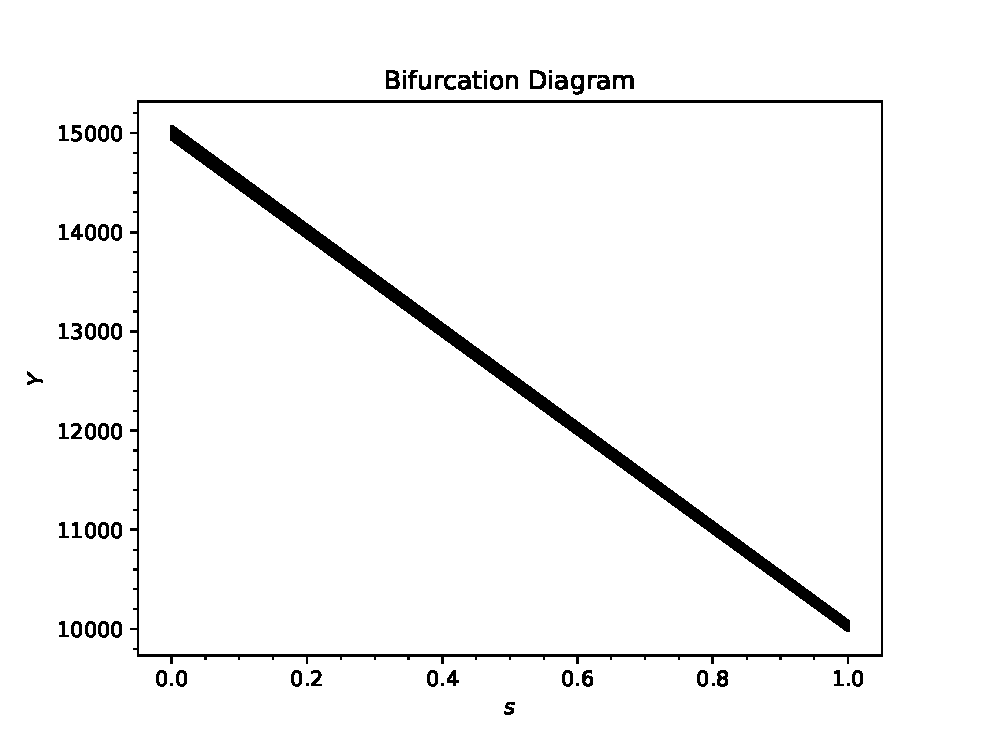
\includegraphics[width=1.2\textwidth]{sbifurcation.eps}
			\caption{Bifurcation diagram varying s}
		\end{figure}
	\end{column}
	\begin{column}{0.5\textwidth}
		\begin{figure}
			\centering
			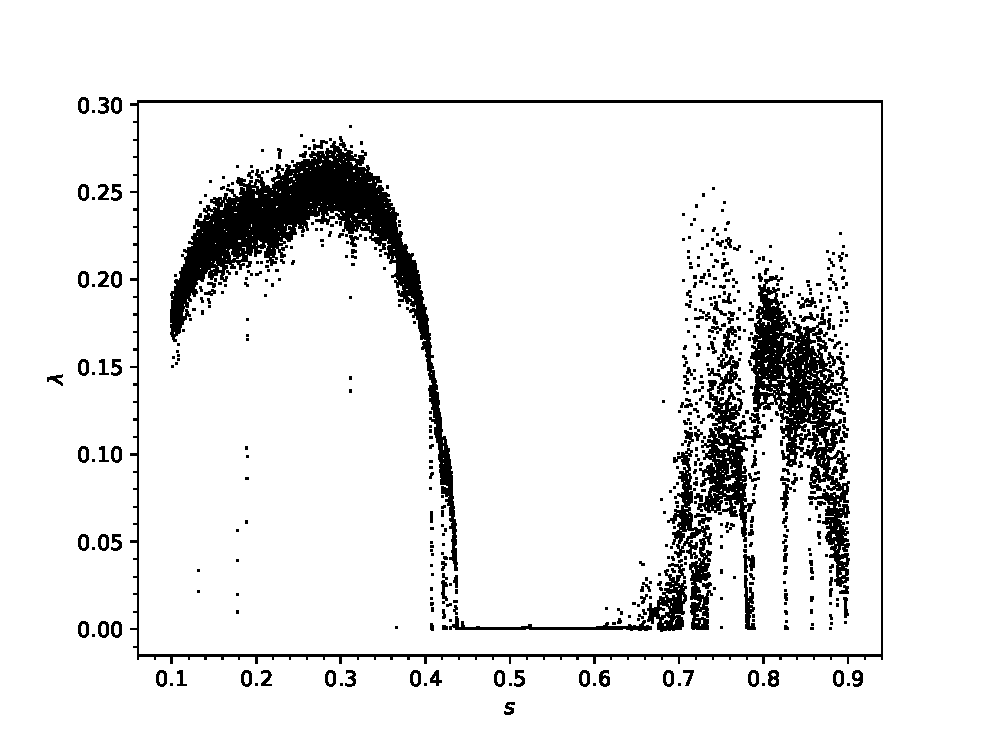
\includegraphics[width=1.2\textwidth]{slyplot.eps}
			\caption{Lyapunov plot varying s}
		\end{figure}
	\end{column}
	\end{columns}
\end{frame}

\begin{frame}{Investment (FWHM): Measured by $v$}
	\begin{columns}
	\begin{column}{0.5\textwidth}
		\begin{figure}
			\centering
			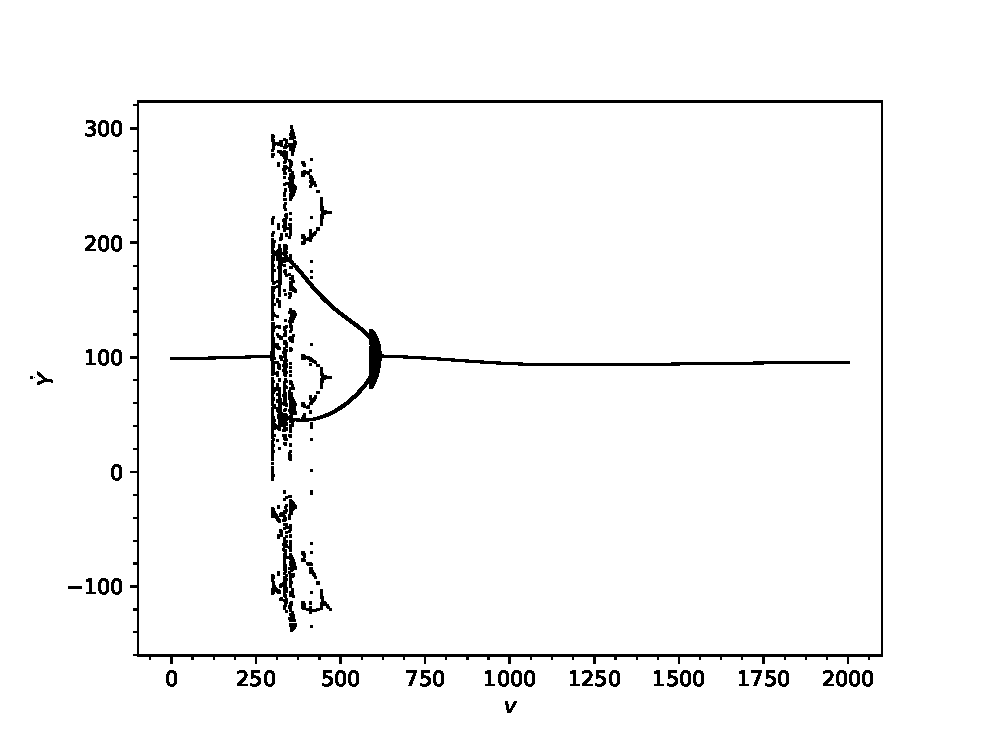
\includegraphics[width=1.2\textwidth]{vbifurcation.eps}
			\caption{Bifurcation diagram varying v}
		\end{figure}
	\end{column}
	\begin{column}{0.5\textwidth}
		\begin{figure}
			\centering
			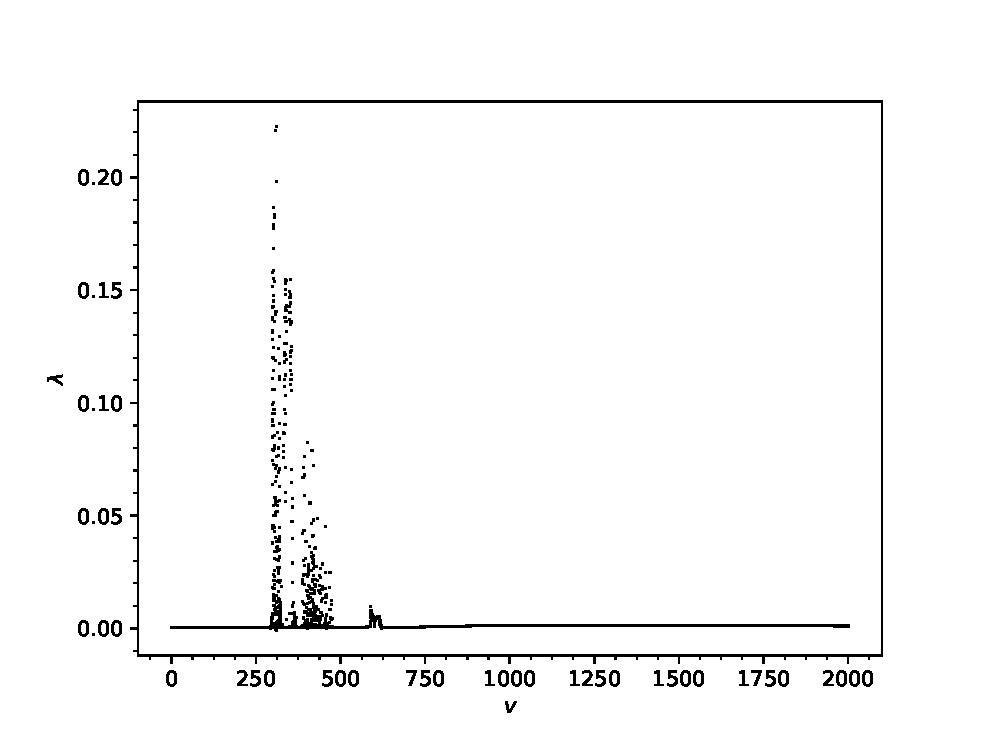
\includegraphics[width=1.2\textwidth]{vlyplot.eps}
			\caption{Lyapunov plot varying v}
		\end{figure}
	\end{column}
	\end{columns}
\end{frame}

\begin{frame}{Investment (Maximum/Minimum): Measured by $q$}
	\begin{columns}
	\begin{column}{0.5\textwidth}
		\begin{figure}
			\centering
			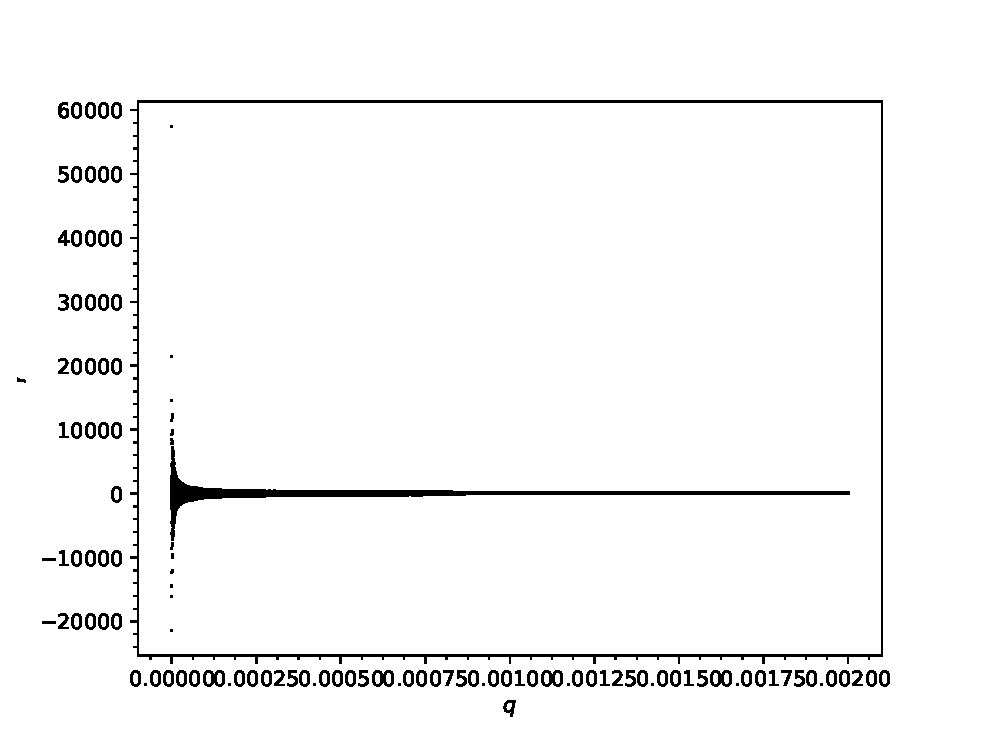
\includegraphics[width=1.2\textwidth]{qbifurcation.eps}
			\caption{Bifurcation diagram varying q}
		\end{figure}
	\end{column}
	\begin{column}{0.5\textwidth}
		\begin{figure}
			\centering
			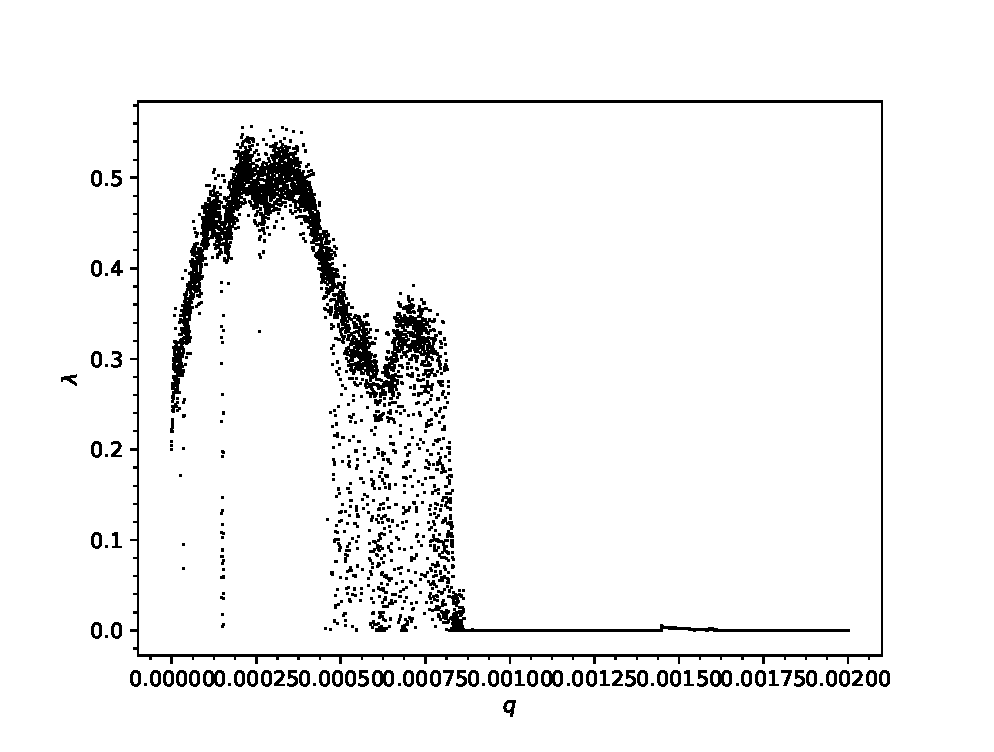
\includegraphics[width=1.2\textwidth]{qlyplot.eps}
			\caption{Lyapunov plot varying q}
		\end{figure}
	\end{column}
	\end{columns}
\end{frame}

\begin{frame}{Sensitivity to Initial Conditions}
	\begin{columns}
	\begin{column}{0.5\textwidth}
		\begin{figure}
			\centering
			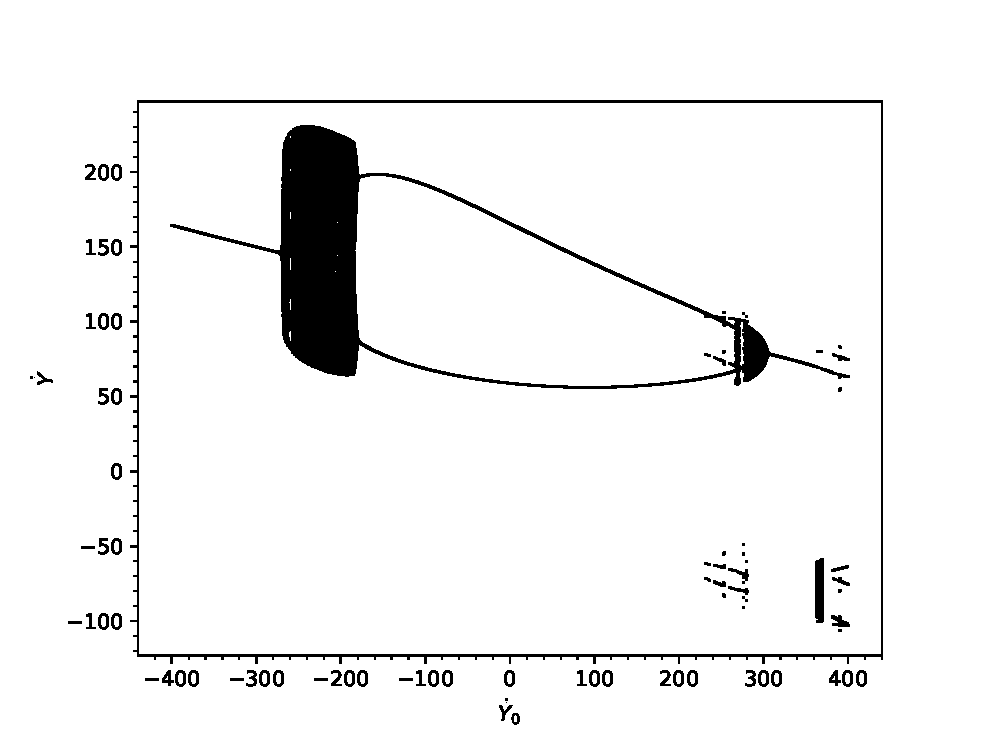
\includegraphics[width=1.2\textwidth]{y0bifurcation.eps}
			\caption{Bifurcation diagram varying $\dot Y_0$}
		\end{figure}
	\end{column}
	\begin{column}{0.5\textwidth}
		\begin{figure}
			\centering
			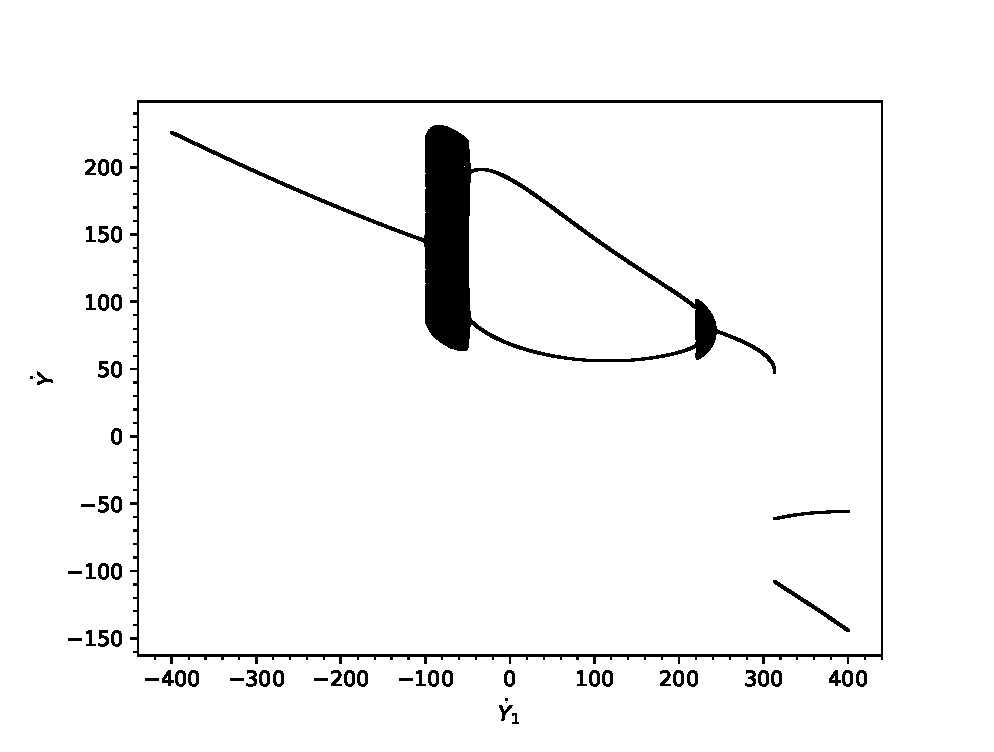
\includegraphics[width=1.2\textwidth]{y1bifurcation.eps}
			\caption{Bifurcation diagram varying $\dot Y_1$}
		\end{figure}
	\end{column}
	\end{columns}
\end{frame}

\begin{frame}{Sensitivity to Initial Conditions}
	\begin{columns}
	\begin{column}{0.5\textwidth}
		\begin{figure}
			\centering
			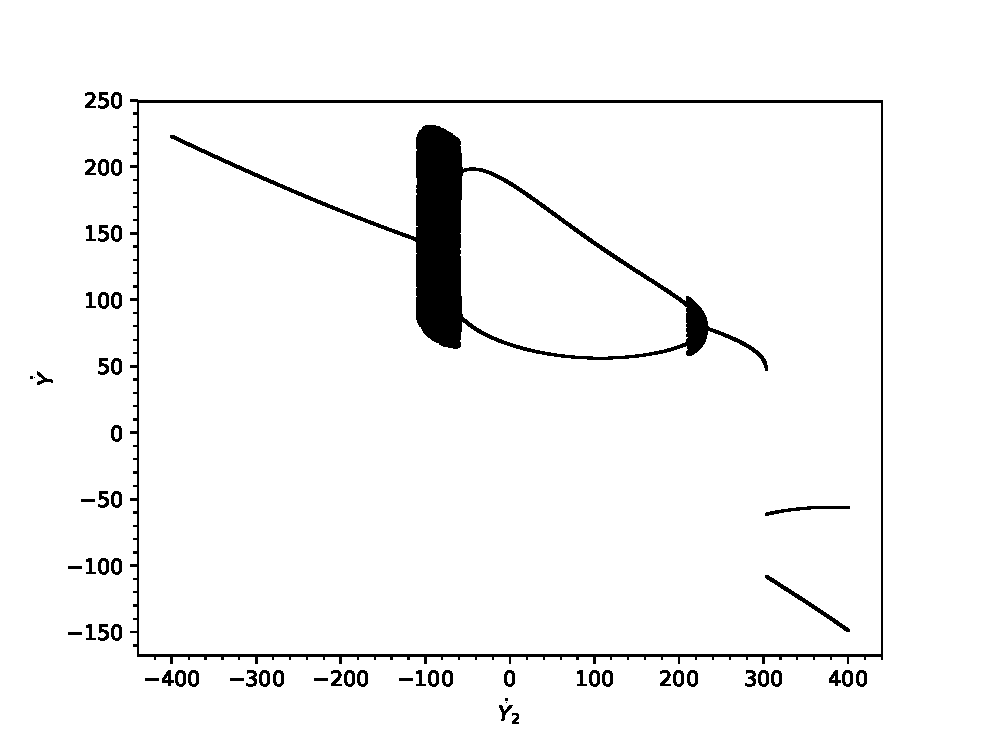
\includegraphics[width=1.2\textwidth]{y2bifurcation.eps}
			\caption{Bifurcation diagram varying $\dot Y_2$}
		\end{figure}
	\end{column}
	\begin{column}{0.5\textwidth}
		\begin{figure}
			\centering
			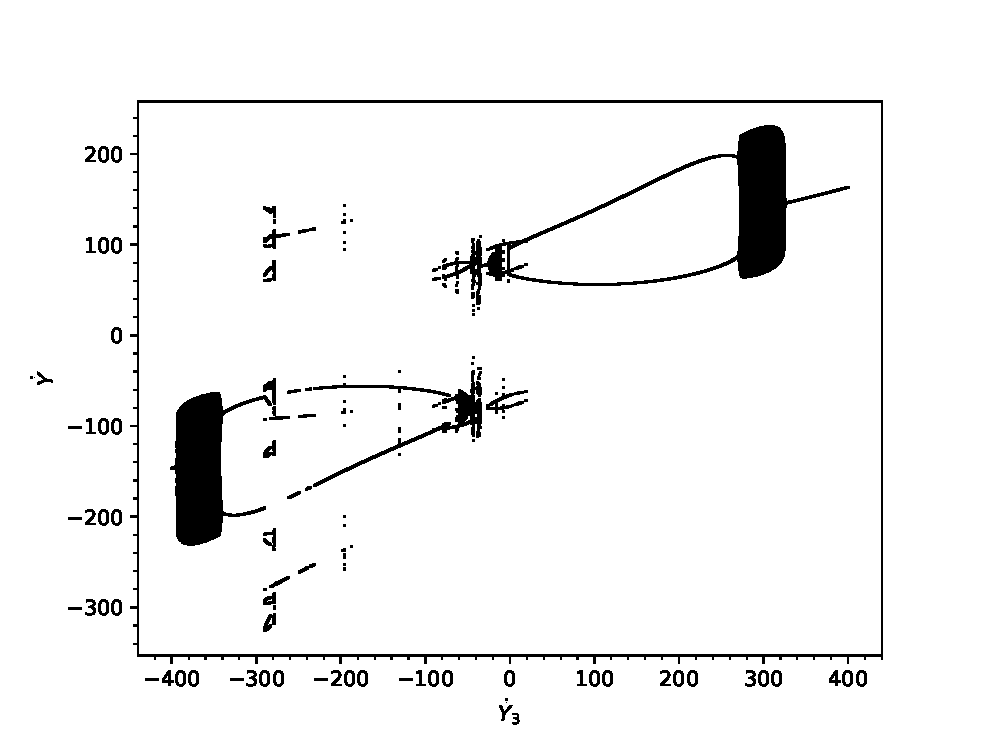
\includegraphics[width=1.2\textwidth]{y3bifurcation.eps}
			\caption{Bifurcation diagram varying $\dot Y_3$}
		\end{figure}
	\end{column}
	\end{columns}
\end{frame}

\begin{frame}{Sensitivity to Initial Conditions}
	\begin{columns}
	\begin{column}{0.5\textwidth}
		\begin{figure}
			\centering
			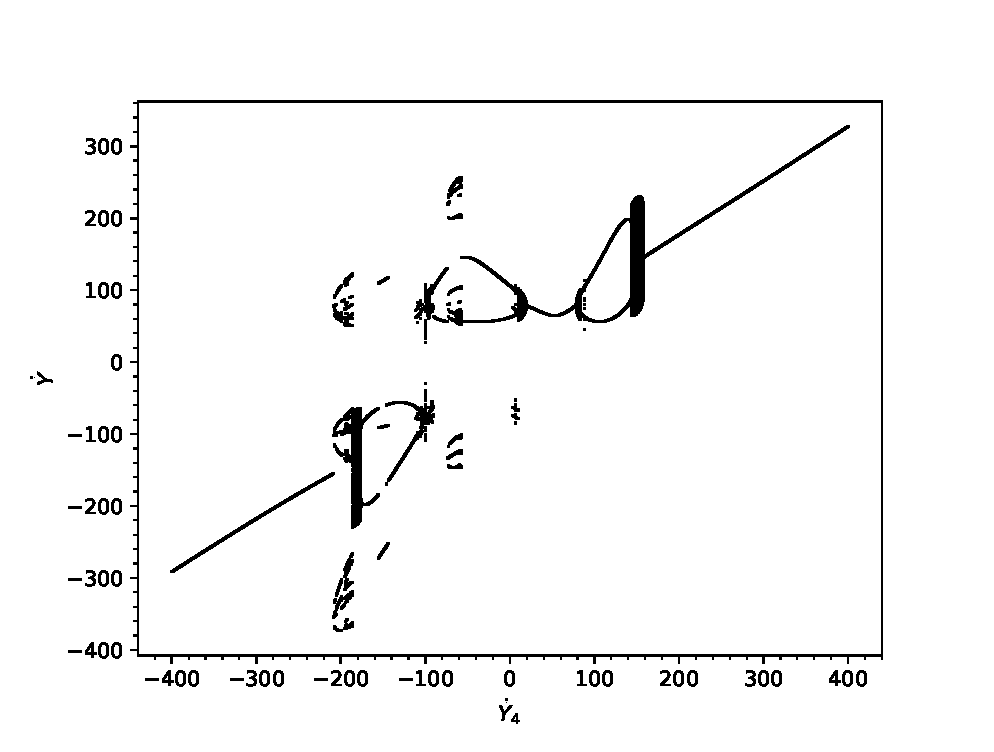
\includegraphics[width=1.2\textwidth]{y4bifurcation.eps}
			\caption{Bifurcation diagram varying $\dot Y_4$}
		\end{figure}
	\end{column}
	\begin{column}{0.5\textwidth}
		\begin{figure}
			\centering
			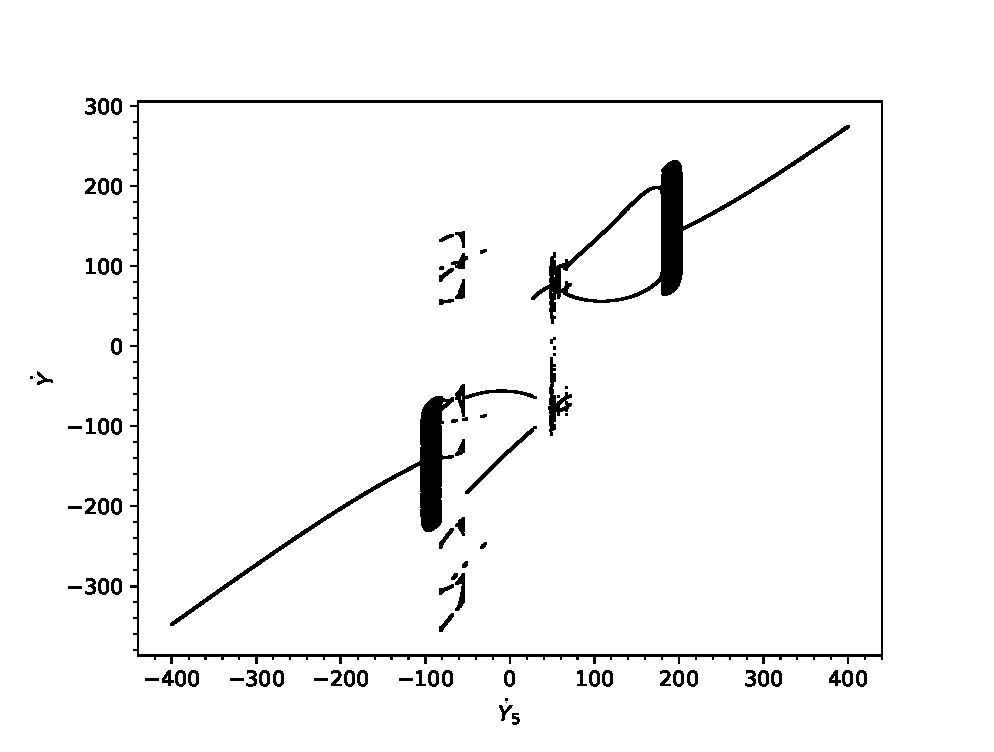
\includegraphics[width=1.2\textwidth]{y5bifurcation.eps}
			\caption{Bifurcation diagram varying $\dot Y_5$}
		\end{figure}
	\end{column}
	\end{columns}
\end{frame}


\begin{frame}{Next steps}
	\begin{itemize}
		\item Further investigate the fractal structure of the strange attractors
		\item Open the economy to foreign trade and improve the investment mechanism 
		\item Improve consumption prediction mechanism
	\end{itemize}
\end{frame}

\begin{frame}[allowframebreaks]{References}
	\nocite{*}
	\printbibliography
\end{frame}
\end{document}
